\section{Results}
% We first report the performance of the classification system, as the system performance greatly impacts the subjective experience of the motor augmentation.

% \subsection{Behavior: Intentional Binding}
In the intentional binding task, i.e. the estimation of the time interval between tap and tone, participants generally underestimated the average real delay (350ms) in all three conditions (INTENTION M = -160.7 ms, SD = 88.1; INVOLUNTARY M = -135.3, SD = 110.3, AUGMENTED M = -162.4, SD = 113.8). The underestimation was not affected by the condition, see~\ref{fig:ib_task}.

% The condition influenced the estimation (${\chi^{2}_{(2)}} = 17.1, p < .001$), see figure~\ref{fig:results}a. Post-hoc tests revealed that the underestimation was less pronounced in INVOLUNTARY as compared to INTENTION ($beta = 22.6, p < 0.001$). This was also the case in INVOLUNTARY, with less pronounced underestimations of the time interval between tap and tone compared to AUGMENTED ($beta = 15.3, p = 0.018$). No difference was observed between INTENTION and AUGMENTED.

\begin{figure}[h]
    \centering
    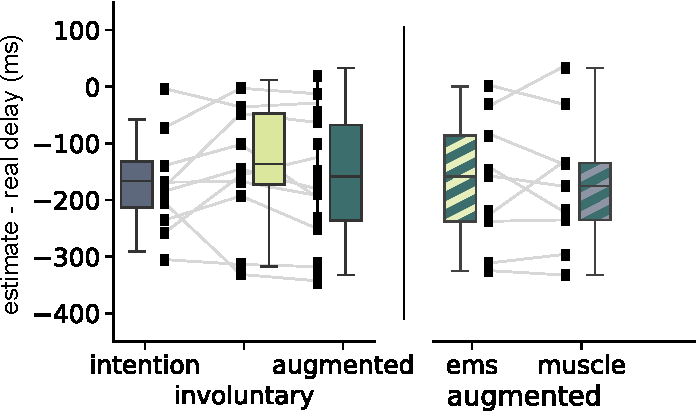
\includegraphics[width=\columnwidth]{figures/ib_task.pdf}
    \caption{Difference in time estimation from real delay in intentional binding task for the three experimental conditions (left). Negative values indicate a temporal compression, i.e., temporal binding. Right side: Trials in the AUGMENTED condition split in EMS-- and self-executed trials.}
    \label{fig:ib_task}
\end{figure}

\subsection{Subjective Ratings \& Reports}
The subjective rating of control differed between conditions (${\chi^{2}_{(2)}} = 43.7, p < .001$), see figure~\ref{fig:loc}b. Post-hoc tests revealed that participants rated their level of control higher in INTENTION compared to INVOLUNTARY ($beta = 4.8, p < .0001$), and higher in INTENTION compared to AUGMENTED ($beta = 3.1, p < .0001$). Further, higher control was observed in AUGMENTED compared to INVOLUNTARY ($beta = -2.9, p = .006$).

% \begin{figure}[h]
%     \centering
%     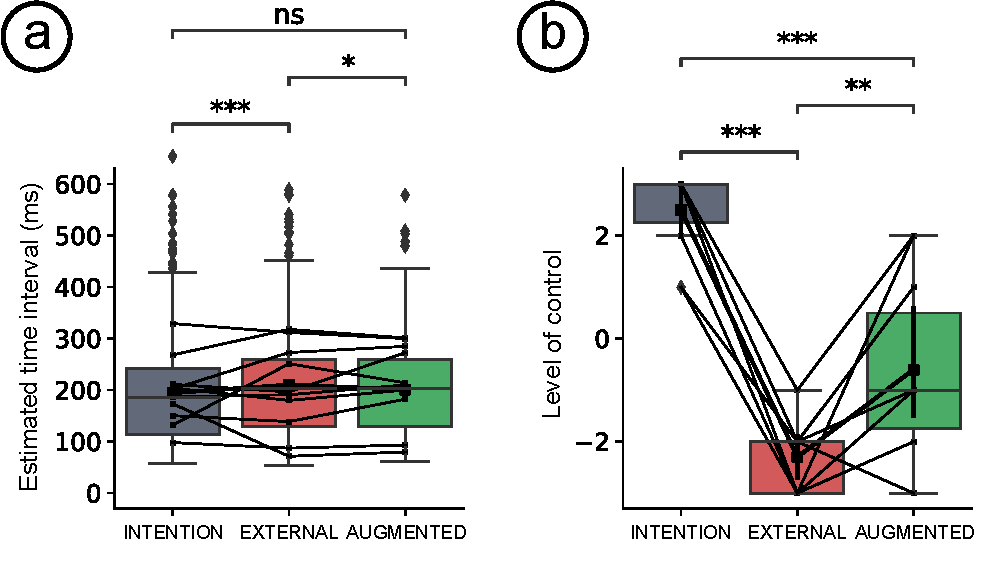
\includegraphics[width=\columnwidth]{figures/subjective_results.pdf}
%     \caption{(a) Temporal binding effect over conditions. With an average presented time interval of 350ms, lower values in the estimated time interval indicate an underestimation, i.e., temporal binding. (b) Subjective ratings of control across conditions. Significance labels obtained from post-hoc tests on estimated marginal means.}
%     \label{fig:results}
% \end{figure}

\begin{figure}[h]
    \centering
    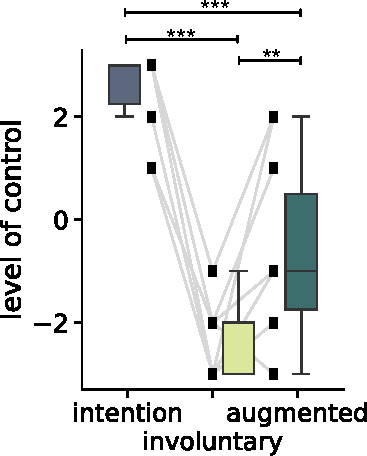
\includegraphics[width=.5\columnwidth]{figures/level_of_control.pdf}
    \caption{Subjective ratings of control across conditions. Significance labels obtained from post-hoc tests on estimated marginal means.}
    \label{fig:loc}
\end{figure}

\paragraph{Functionality.} Eight out of the ten participants made a reference to the source of the EMS in the AUGMENTED condition. In that subgroup, most participants wondered how the system worked, one remarked, ``I can't explain how it works technically.''. Another one mentioned that ``maybe the time estimation task had something to do with it.''. They found the stimulation to be sporadic, even during their own actions, leading to a belief that it was coincidental. As one participant put it, ``I have no idea what controlled the stimulation, I think it was coincidence when stimulation occurred.''. Furthermore, participants reported that they found the timing of the stimulation to be unpredictable, with one participant noting, ``Stimulation was random in time.''. 

Some perceived the stimulation as externally triggered, yet partially responsive to their choices, resulting in a sentiment captured by, ``I think that the stimulation in the third block was partly random, but partly as if it was following my decision/choice.''. One participant noted that they felt that ``somehow the information is in my arm''. Another one briefly considered the involvement of their brain waves in controlling the stimulation, but expressed doubts about this possibility, stating, ``But I don't think that is the case.''.

\paragraph{Guessed Percentage.} 
Some participants reported that the stimulation ``sometimes overlapped with the movement, but not often,'' or, it ``came only rarely.'' Another one noted, ``In a few cases, the stimulation came when I had already started the movement.'' For several participants, this overlap between their actions and the system's response occurred infrequently, with another user noting, ``Once, in the millisecond range between my planned movement and its execution.'' However, for some participants, there were moments of near-perfect synchronization, as described by one participant, ``In 3 cases it happened that my intention to press and the impulse of the device happened simultaneously.'' or ``in 3--4 cases it happened simultaneously that i wanted to tap and the stimulation happened''. Another one noted, ``Sometimes it really happened that they overlapped. So that I just started to move, and then the device activated,'' that user estimated an overlap of ``40 \%'' while two other users said [we worked together in] ``15 \% of trials.'' These accounts collectively highlight the varied and occasionally synchronous nature of the system's timing in relation to the users' intentions.

\paragraph{Correct Interaction.} 
In terms of valence sentiments for the cases where the stimulation aligned with participants' intentions, some participants indicated that the experience was positive, for example, participants described the experience as ``rather funny'', ``weird but funny'', ``pleasant'' or ``helped me with the execution'' and ``it was more of a collective movement.'' One participant remarked ``then it was ok to experience the stimulation, but also not more than ok'' while another one noted ``It had a bit of thinking ahead to it''. Some noted that they experienced an increase in their physical strength, remarking, ``supported my strength'', ``made me type more firmly'' and ``my typing performance was increased.'' On the other hand, some participants had negative sentiments during these moments of aligned stimulation, remarking, ``felt like I was still in competition with the system'', ``it did not feel like an acting together'' and ``on a psychological level it was a loss of control.'' Another one noted, that they ``felt determined-by-others and then tried to resist the impulse. I felt excluded from the decision to tap''.

\subsection{Classifier Performance}
Visual inspection of the amplitudes at electrode Cz revealed an increase in the difference between \textit{pre-movement} and \textit{idle} data segments towards the onset of the finger movement, see figure~\ref{fig:EEG_results}a. The slope feature for the exemplary channel Cz discriminates well between the two classes (${t_{(10)}} = 4.4, p < .001$), see figure ~\ref{fig:EEG_results}b bottom. The scalp maps in figure~\ref{fig:EEG_results}b top show the (color-coded) mean slope for each channel and each class. Central channels on the contralateral side to the moving finger on the right hand show a negative slope for the pre-movement class and a neutral slope for the idle class. Furthermore, differences in slope were also observed at frontal electrodes over the left hemisphere as well as parietal electrodes, were a positive slope manifested only for the idle class. 

\begin{figure*}[t]
    \centering
    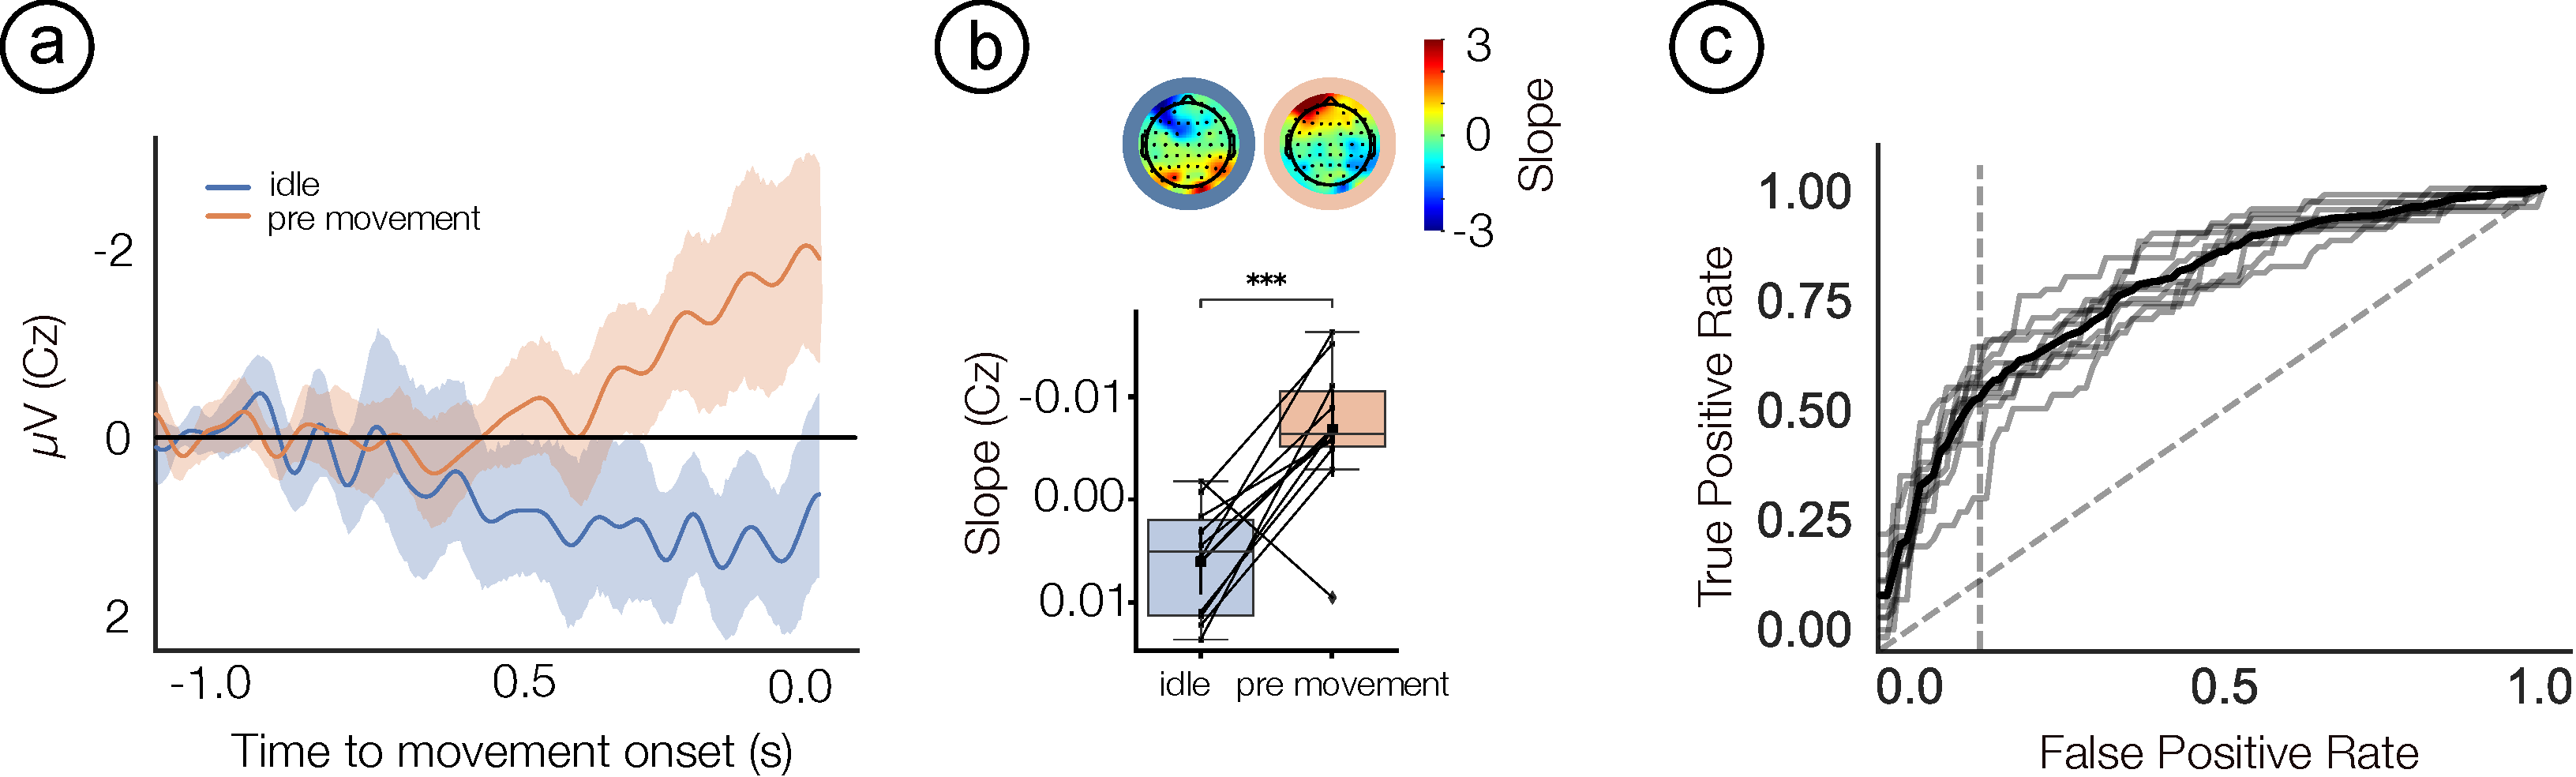
\includegraphics[width=\textwidth]{figures/eeg_results_new.pdf}
    \caption{(a) Grand average event-related potential (ERP) at electrode Cz of pre-movement EEG data epochs preceding the last second before a movement, idle epochs of the same trial are plotted alongside but originate from a different time window, see section~\ref{eeg_methods}; (b) Bottom: Slope features for both idle and pre-movement classes at electrode Cz. Top: Scalp maps of slope values for both classes and all channels. (c): Mean and per participant ROC curves. Dotted line at 15 \% false positive rate indicate the selected threshold for the real-time application.}
    \label{fig:EEG_results}
\end{figure*}

The grid-search over channels resulted in the BCI leveraging on average 11.2 (SD = 3.6) channels. Besides channels C3, C4, and Cz, that were always included, other common channels (retained for at least 3 participants) included FT9 and AF3. The classifier cross-validation resulted in a mean F1 score of .71 (SD = .03), see figure~\ref{fig:EEG_results}c. We set the detection threshold to 15 \% false positive rate and at that rate, observed a mean threshold of 57 \% (SD = .04). Hence, on average, the classifier switched on the EMS when it predicted class \textit{pre-movement} with 57 \% probability.

\subsubsection{Post-hoc analyses of classifier performance}

In line with the readiness potential a negative going deflection over the last second preceding the movement onset was present in both INTENTION and AUGMENTED, but not in INVOLUNTARY, see figure~\ref{fig:erp}a. Furthermore, ERPs differed between the three conditions in the time window from 210 ms -- 250 ms following movement onset ($\chi^{2}_{(2} = 10.6, p = .03$ at 220 ms). INVOLUNTARY exhibited a strong negativity peak (strongest among the three conditions), peaking at around -10 $\mu$V at 210 ms after movement onset. A weaker peak was observed for AUGMENTED (-6 $\mu$V at 210 ms) and even more so for INTENTION (-2 $\mu$V at 150 ms).

\begin{figure}[h]
    \centering
    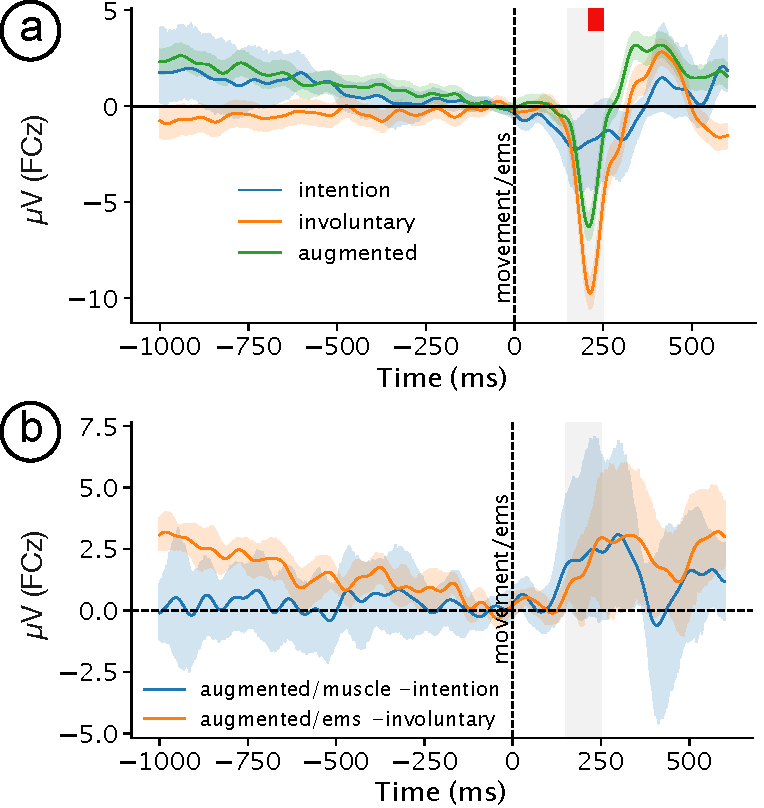
\includegraphics[width=\columnwidth]{figures/PE_erp.pdf}
    \caption{ERPs at electrode FCz from -1000 before, to 600 ms after the tapping movement onset. Top (a): INTENTION, INVOLUNTARY and AUGMENTED trials. Red bar on top indicate main effect at $p<.05$. Bottom (b): Difference ERPs at FCz of the `muscle-controlled' trials in AUGMENTED minus INTENTION as well as EMS trials in AUGMENTED minus INVOLUNTARY.}
    \label{fig:erp}
\end{figure}

When correcting for the influence of the EMS by subtracting INVOLUNTARY from EMS trials in AUGMENTED an INTENTION from `muscle-controlled' trials in AUGMENTED we observed no differences. Visually, it appears that trials in both INVOLUNTARY and INTENTION condition exhibit a stronger negativity in the post movement time window of interest than respective EMS and `muscle-controlled' trials in AUGMENTED, see the positive deflections peaking at 300 ms post movement onset in figure~\ref{fig:erp}b.



%%% Resources and Ideas
% and the agency condition by xx (CI: ). Subsequent non-parametric comparisons revealed the significance of differences only between  
% xx (p = ).
% x\



%\missingfigure{A: Boxplot of questionnaire scores of three Blocks (block 2 grey, because not intention given) - play around with visualization of words that were used to explain control rating. B. Boxplots intentional binding (maybe integrate A and B) C. more subjective evaluation of interview / maybe world cloud / maybe sentiment analysis) } 



% Did they get faster? Calculate time between hand motion onset and button press. If yes, evidence that there was acceptance for the help/augmentation the system provided
